\setcounter{figure}{0}
\renewcommand{\thefigure}{\Alph{figure}}
\setcounter{table}{0}
\renewcommand{\thetable}{\Alph{table}}



\section{Appendix}



\subsection{Additional Qualitative Comparison}
\label{supp:additional_qualitative}

We present additional qualitative results on Stereo4D (\cref{fig:supp:qual_stereo4D}), KITTI (\cref{fig:supp:qual_kitti}), and Bonn (\cref{fig:supp:qual_bonn}).
Our method consistently shows more accurate depth and motion estimates than competing approaches.
A notable advantage is our robustness to significant camera rotation and object motion (\eg the first two rows in \cref{fig:supp:qual_stereo4D}), where other methods often produce erroneous estimates.
Furthermore, our method effectively disentangles dynamic object motion from camera ego-motion, successfully isolating moving objects where other methods frequently assign non-zero motion to static backgrounds.
Unlike the blurred predictions seen in DynaDUSt3R, our method preserves sharp motion boundaries and geometric consistency across all datasets.




\begin{figure*}[!h]
\centering
\scriptsize
\setlength\tabcolsep{0.2pt}
\newcommand{\qualimgjpg}[3]{\includegraphics[width=0.155\textwidth]{figure/qual/main/#1/#2/#3.jpg}}
\newcommand{\qualimgpng}[3]{\includegraphics[width=0.15\textwidth]{figure/qual/main/#1/#2/#3.png}}

\newcommand{\ablqualrow}[2]{
\qualimgpng{#1}{#2}{img0} & 
\rotatebox{90}{Depth} &
\qualimgpng{#1}{#2}{d_dy} & 
\qualimgpng{#1}{#2}{d_zm} &
\qualimgpng{#1}{#2}{d_st} &
\qualimgpng{#1}{#2}{d_ours} & 
\qualimgpng{#1}{#2}{d_gt} 
\\
\qualimgpng{#1}{#2}{img1} & 
\rotatebox{90}{Motion} &
\qualimgpng{#1}{#2}{m_dy} & 
\qualimgpng{#1}{#2}{m_zm} &
\qualimgpng{#1}{#2}{m_st} &
\qualimgpng{#1}{#2}{m_ours} & 
\qualimgpng{#1}{#2}{m_gt}
}

\newcolumntype{M}{>{\centering\arraybackslash}m{0.155\textwidth}}
\newcolumntype{N}{>{\centering\arraybackslash}m{0.02\textwidth}}

\begin{tabular}{M @{\hspace{0.8em}} N M M M M M}
    \ablqualrow{stereo4d}{MhxqBDWonRw-clip137-frame_21_43} \\ \noalign{\smallskip}
    \ablqualrow{stereo4d}{CLsVoV-9OrI-clip6-frame_5_29} \\ \noalign{\smallskip}
    \ablqualrow{stereo4d}{tPwC06dft1w-clip31-frame_3_18} \\ \noalign{\smallskip}
    Input pair & & \makecell[c]{DynaDUSt3R \\ \cite{Jin:2025:S4D}}& \makecell[c]{ZeroMSF \\ \cite{Liang:2025:ZSM}} & \makecell[c]{St4RTrack \\ \cite{Feng:2025:ST4}} & \textbf{\ourmethod{} (Ours)} & Ground truth \\
\end{tabular}
\caption{
\textbf{Qualitative comparison on Stereo4D.} We visualize depth and projected 2D optical flow. UFO-4D consistently outperforms other methods in depth and motion accuracy. Notably, in scenes with significant camera rotation (top two rows), our method robustly estimates 3D geometry and isolates 3D motion of dynamic objects in the canonical space. In contrast, other methods struggle to disentangle camera ego-motion, resulting in residual motion artifacts on static background.
\label{fig:supp:qual_stereo4D}
}
\end{figure*}


\begin{figure*}[t]
\centering
\scriptsize
\setlength\tabcolsep{0.2pt}
\newcommand{\qualimgjpg}[3]{\includegraphics[width=0.155\textwidth]{figure/qual/main/#1/#2/#3.jpg}}
\newcommand{\qualimgpng}[3]{\includegraphics[width=0.15\textwidth]{figure/qual/main/#1/#2/#3.png}}

\newcommand{\ablqualrowkitti}[2]{
\qualimgpng{#1}{#2}{img0} & 
\rotatebox{90}{Depth} &
\qualimgpng{#1}{#2}{d_dy} & 
\qualimgpng{#1}{#2}{d_zm} &
\qualimgpng{#1}{#2}{d_st} &
\qualimgpng{#1}{#2}{d_ours} & 
\qualimgpng{#1}{#2}{d_gt} 
\\
\qualimgpng{#1}{#2}{img1} & 
\rotatebox{90}{Motion} &
\qualimgpng{#1}{#2}{m_dy} & 
\qualimgpng{#1}{#2}{m_zm} &
\qualimgpng{#1}{#2}{m_st} &
\qualimgpng{#1}{#2}{m_ours} &
\qualimgpng{#1}{#2}{m_gt}
}

\newcolumntype{M}{>{\centering\arraybackslash}m{0.155\textwidth}}
\newcolumntype{N}{>{\centering\arraybackslash}m{0.02\textwidth}}

\begin{tabular}{M @{\hspace{0.8em}} N M M M M M}
    \ablqualrowkitti{kitti}{000022_10} \\ \noalign{\smallskip}
    \ablqualrowkitti{kitti}{000046_10} \\ \noalign{\smallskip}
    \ablqualrowkitti{kitti}{000077_10} \\ \noalign{\smallskip}
    \ablqualrowkitti{kitti}{000090_10} \\ \noalign{\smallskip}
    \ablqualrowkitti{kitti}{000190_10} \\ \noalign{\smallskip}
    Input pair & & \makecell[c]{DynaDUSt3R \\ \cite{Jin:2025:S4D}}& \makecell[c]{ZeroMSF \\ \cite{Liang:2025:ZSM}} & \makecell[c]{St4RTrack \\ \cite{Feng:2025:ST4}} & \textbf{\ourmethod{} (Ours)} & Ground truth \\
\end{tabular}
\caption{
    \textbf{Qualitative comparison on KITTI.} We visualize motion in camera coordinates, consistent with the ground truth of KITTI. Our method outperforms competitors with notably clearer motion boundaries, whereas ZeroMSF and St4RTrack frequently show erroneous motion estimation.
    \label{fig:supp:qual_kitti}
}
\end{figure*}


\begin{figure*}[!th]
\centering
\scriptsize
\setlength\tabcolsep{0.2pt}
\newcommand{\qualimgjpg}[3]{\includegraphics[width=0.155\textwidth]{figure/qual/main/#1/#2/#3.jpg}}
\newcommand{\qualimgpng}[3]{\includegraphics[width=0.15\textwidth]{figure/qual/main/#1/#2/#3.png}}

\newcommand{\ablqualrowbonn}[2]{
\qualimgpng{#1}{#2}{img0} & 
\rotatebox{90}{Depth} &
\qualimgpng{#1}{#2}{d_dy} & 
\qualimgpng{#1}{#2}{d_zm} &
\qualimgpng{#1}{#2}{d_st} &
\qualimgpng{#1}{#2}{d_ours} &
\qualimgpng{#1}{#2}{d_gt} 
\\
\qualimgpng{#1}{#2}{img1} & 
\rotatebox{90}{Motion} &
\qualimgpng{#1}{#2}{m_dy} & 
\qualimgpng{#1}{#2}{m_zm} &
\qualimgpng{#1}{#2}{m_st} &
\qualimgpng{#1}{#2}{m_ours} &
(N/A)
}

\newcolumntype{M}{>{\centering\arraybackslash}m{0.155\textwidth}}
\newcolumntype{N}{>{\centering\arraybackslash}m{0.02\textwidth}}

\begin{tabular}{M @{\hspace{0.8em}} N M M M M M}
    \ablqualrowbonn{bonn}{rgbd_bonn_crowd2_1548339893.24032_1548339893.57482} \\ \noalign{\smallskip}
    \ablqualrowbonn{bonn}{rgbd_bonn_crowd3_1548339961.77666_1548339962.11179} \\ \noalign{\smallskip}
    \ablqualrowbonn{bonn}{rgbd_bonn_person_tracking2_1548265922.17945_1548265922.51462} \\ \noalign{\smallskip}
    Input pair & & \makecell[c]{DynaDUSt3R \\ \cite{Jin:2025:S4D}}& \makecell[c]{ZeroMSF \\ \cite{Liang:2025:ZSM}} & \makecell[c]{St4RTrack \\ \cite{Feng:2025:ST4}} & \textbf{\ourmethod{} (Ours)} & Ground truth \\
\end{tabular}
\caption{
\textbf{Qualitative comparison on Bonn.}
Comparing to other methods, our method outputs clear 3D motion disentangled from camera motion. ZeroMSF and St4RTrack suffer from non-zero residual motion in background. DynaDUSt3R tends to show unclear motion boundaries.
\label{fig:supp:qual_bonn}
}
\end{figure*}




\subsection{Evaluation protocol}
\label{sec:app:inference_setup}
In \cref{sec:exp:eval_2d_3d}, we compare our method with direct competitors, \eg, DynaDUSt3R~\citep{Jin:2025:S4D}, ZeroMSF~\citep{Liang:2025:ZSM}, and St4RTrack~\citep{Feng:2025:ST4}, that output point and 3D scene flow.
Due to that each method has their own inference setups, we include details here on their evaluation setups used in our comparison study.

\paragraph{DynaDUSt3R.} 
Similar to our method, DynaDUSt3R~\citep{Jin:2025:S4D} outputs pointmaps and scene flow in the first frame's coordinate system, allowing us to use its predictions directly.
For inference, we resize inputs to $512\times512$ for Stereo4D and Bonn.
For KITTI and Sintel, we use resize inputs to $382\times512$ following their protocol and $208\times512$ preserving aspect ratio, respectively.
All outputs are resized back to the original resolution for evaluation.

\paragraph{ZeroMSF.}
We use the same inference resolution as in DynaDUSt3R~\citep{Jin:2025:S4D}.
While ZeroMSF~\citep{Liang:2025:ZSM} defines pointmaps in the first camera coordinate, it parameterizes scene flow as Camera-space 3D offsets (CSO)—estimating motion relative to a fixed camera.
To ensure fair comparison on datasets where their motion is defined at the canonical camera coordinate (Stereo4D), we convert this flow to world coordinates using ground truth extrinsics. Although using ground truth poses grants ZeroMSF an advantage, it is necessary to minimize errors arising from coordinate system mismatch. 

\paragraph{MASt3R, MonST3R, and St4RTrack.}
For MASt3R, MonST3R, and St4RTrack, we follow the original evaluation protocol in their implementation. 
Unlike our method, MonST3R and St4RTrack do not directly output relative camera pose in a feedforward manner.
For the pose estimation, we use a PnP solver with RANSAC with their default hyperparameters. 



\subsection{Some observations about the Stereo4D dataset}

Stereo4D~\citep{Jin:2025:S4D} provides a large-scale annotated data for 4D understanding, specifically including camera intrinsics, extrinsics, depth, 3D point trajectory. 
While it is the biggest real-world based annotated dataset, we found that it includes noisy annotations that residuals from its optimization process given depth and motion cues processed from off-the-shelf models.
\cref{fig:stereo4d_dataset} visualizes some samples from Stereo4D.
The last column visualizes motion map in the standard optical flow color coding.
Close examination shows that some static region (\eg, ground and building wall) include non-zero motion, which is typically under centimeter level.

This noisy annotation may result in non-zero motion estimates for static parts, as visualized in \cref{fig:qualitative_main} for DynaDust3R.
Our dense, self-supervised photometric loss on rendered images complements the imperfect ground truth and lead to better motion accuracy than other methods. 
% \ds{If GT is wrong for static parts, the eval numbers are not one hundred percent correct.}


\begin{figure*}[!t]
\centering
\footnotesize
\setlength\tabcolsep{1pt}
\newcommand{\vizstereodataset}[1]{
\includegraphics[width=0.22\textwidth]{figure/analyses/stereo4d_viz/#1_img0.png} &
\includegraphics[width=0.22\textwidth]{figure/analyses/stereo4d_viz/#1_img1.png} &
\includegraphics[width=0.22\textwidth]{figure/analyses/stereo4d_viz/#1_motion.png}
}
\begin{tabular}{ccc}
\vizstereodataset{1} \\
\vizstereodataset{2} \\
\vizstereodataset{3} \\
First image & Second image & Visualized 3D motion \\
\end{tabular}


\caption{\textbf{Visualization of annotation of Stereo4D.} The first two columns visualize two input frames, and the last columns visualizes 3D motion annotation defined at the canonical camera coordinate. While Stereo4D provides large-scale real-world annotated data, the label includes noisy annotation, \eg, non-zero 3D motion for static region.
}
\label{fig:stereo4d_dataset}
\end{figure*}


\begin{table}[t]
\centering
\scriptsize
\setlength\tabcolsep{1pt}
\caption{\textbf{Geometry estimation (under per-valid-pixel averaging protocol)}: Using the same evaluation metric in DynaDUSt3R, our method consistently outperforms other methods.}
\label{tab:exp:depth_pervalid}
\newcolumntype{Y}{S[table-format=1.3, round-mode=places, round-precision=3]}
\newcolumntype{Z}{S[table-format=2.2, round-mode=places, round-precision=2]}
\begin{tabularx}{\linewidth}{@{} X @{\hskip 0.2em} *{4}{@ {\hskip 0.1em} Y Y Z} @{}}
\toprule
\multirow{2}{*}{Method} & \multicolumn{3}{c}{Stereo4D}  & \multicolumn{3}{c}{Bonn}  & \multicolumn{3}{c}{KITTI} & \multicolumn{3}{c}{Sintel final}\\
\cmidrule(r){2-4} \cmidrule(r){5-7} \cmidrule(r){8-10} \cmidrule(r){11-13}
& {EPE} & {Abs.~Rel.} & {$\delta{\lt} 1.25$} & {EPE} & {Abs.~Rel.} & {$\delta{\lt} 1.25$} & {EPE} & {Abs.~Rel.} & {$\delta{\lt} 1.25$} & {EPE} & {Abs.~Rel.} & {$\delta{\lt} 1.25$} \\
\midrule
MASt3R~\citep{Leroy:2024:GIM} & 1.6575 & 0.2897 & 65.5990 & 0.4839 & 0.1726 & 76.6771 & \bfseries 2.2467 & \bfseries 0.0856 & \underline{92.15} & 3.9065 & 0.3595 & 60.6771 \\
MonST3R~\citep{Zhang:2025:MST} & 1.3798 & 0.1939 & 72.5653 & 0.1871 & \bfseries 0.0616 & \bfseries 96.2591 & 2.741 & 0.1057 & 87.9555 & \bfseries 3.5138 & 0.3376 & 57.2272 \\
DynaDUSt3R~\citep{Jin:2025:S4D} & \underline{0.683} & \bfseries 0.103 & \underline{87.94} & 0.4230 & 0.0835 & 92.8303 & 4.8054 & 0.1125 & 84.0951 & 4.2958 & \bfseries 0.2946 & 60.8804 \\
ZeroMSF~\citep{Liang:2025:ZSM} & 1.6737 & 0.2412 & 72.7655 & 0.2067 & 0.0782 & 91.6802 & 3.2652 & 0.103 & \bfseries 92.6609 & \underline{3.560} & 0.3266 & \bfseries 63.8047 \\
St4RTrack~\citep{Feng:2025:ST4} & 1.2691 & 0.1975 & 71.3659 & \underline{0.180} & 0.0669 & 95.2358 & 4.6610 & 0.1236 & 83.1346 & 4.0965 & 0.3493 & 56.8702 \\
\textbf{\ourmethod{} (Ours)} & \bfseries 0.5939 & \bfseries 0.1030 & \bfseries 88.1954 & \bfseries 0.1615 & \underline{0.064} & \underline{96.08} & \underline{2.485} & \underline{0.088} & 89.41 & 3.8275 & \underline{0.317} & \underline{61.45} \\
\bottomrule
\end{tabularx}
\end{table}


\begin{table}[!ht]
\centering
\scriptsize
\setlength\tabcolsep{6pt}
\caption{\textbf{Motion estimation (under per-valid-pixel averaging protocol)} We evaluate the scene flow accuracy on the Stereo4D test split \citep{Jin:2025:S4D} and KITTI Scene Flow 2015 Training \citep{Menze:2018:OSF}. Our approach consistently outperforms others on all metrics.}
\label{tab:exp:scene_flow_pervalid}
\begin{tabularx}{0.8\linewidth}{@{} X @{\hskip 4em} *{6}{S[table-format=1.3] S[table-format=2.2]} @{}}
\toprule
\multirow{2}{*}{Method} & \multicolumn{4}{c}{Stereo4D} &
\multicolumn{2}{c}{KITTI} \\
\cmidrule(lr){2-5} \cmidrule(lr){6-7} 
& \multicolumn{2}{c}{forward} & \multicolumn{2}{c}{backward} & \multicolumn{2}{c}{forward} \\
 \cmidrule(lr){2-3} \cmidrule(lr){4-5} \cmidrule(lr){6-7}
& {$\text{EPE}_\text{3D}$} & 
{$\delta^{0.05}_\text{3D}$} & {$\text{EPE}_\text{3D}$} & 
{$\delta^{0.05}_\text{3D}$} & {$\text{EPE}_\text{3D}$} & 
{$\delta^{0.05}_\text{3D}$} \\
\midrule
DynaDUSt3R \citep{Jin:2025:S4D} & 0.118 & 65.19 & \underline{0.106} & \underline{64.47} & 0.467 & 1.09 \\
ZeroMSF \citep{Liang:2025:ZSM} & \underline{0.067} & \underline{67.38} & {--} & {--} & \underline{0.452} & \underline{13.84} \\
St4RTrack \citep{Feng:2025:ST4} &  0.233 & 42.56 & {--} & {--} & 0.768 & 3.36 \\
\textbf{\ourmethod{} (Ours)} & \bfseries 0.023 & \bfseries 91.78 & \bfseries 0.025 & \bfseries 91.28 & \bfseries 0.139 & \bfseries 46.71 \\
\bottomrule
\end{tabularx}
\end{table}



\subsection{Evaluation with Per-valid-pixel Averaging}

While the main paper reports metrics using per-frame averaging (where each frame is weighted equally), an alternative protocol used by DynaDUSt3R~\citep{Jin:2025:S4D} is per-valid-pixel averaging. This approach weights each frame's contribution by its number of valid pixels. For a comprehensive comparison, we report results using this metric as well. Under this per-valid-pixel evaluation, \ourmethod{} also consistently outperforms other baselines on Stereo4D and KITTI and perform very competitive on Bonn and Sintel final, as shown in \cref{tab:exp:depth_pervalid,tab:exp:scene_flow_pervalid}.





\begin{table}[t]
\centering
\scriptsize
\caption{\textbf{Dataset ablation.} Given three training datasets, Stereo4D (ST), PointOdyssey (PO), and Virtual KITTI 2 (VK), we try a different mixture of each dataset, train our model, and report performance on three evaluation datasets, Stere4D, KITTI, and Bonn, reporting PSNR for image reconstruction and end-point error (EPE) for point and motion.
The best accuracy on Stereo4D is achieved by solely training on Stereo4D. Adding Virtual KITTI2 improves especially motion accuracy on KITTI but hurts point accuracy on Bonn. Adding PointOdyssey improves accuracy on Bonn but hurt that on KITTI as trade-off.
All experiment is done in a small scale training.}
\label{tab:exp:data_ablation}
\begin{tabularx}{\linewidth}{@{}X X X @{\hskip 1em} *{2}{S[table-format=2.3] S[table-format=1.3] S[table-format=1.3]} S[table-format=2.3] S[table-format=1.3]  @{}}
\toprule
\multicolumn{3}{l}{Dataset proportion} & \multicolumn{3}{c}{Stereo4D} & \multicolumn{3}{c}{KITTI} & \multicolumn{2}{c}{Bonn} \\
\cmidrule(lr){1-3} \cmidrule(lr){4-6} \cmidrule(lr){7-9} \cmidrule(lr){10-11}
ST & PO & VK & {Image ($\uparrow$)} & {Point ($\downarrow$)} & {Motion ($\downarrow$)} & {Image ($\uparrow$)} & {Point ($\downarrow$)} & {Motion ($\downarrow$)}& {Image ($\uparrow$)} & {Point ($\downarrow$)} \\
\midrule
0.7 &0.15&0.15 & 23.547 & 0.065 & 0.891 & \underline{18.845} & \underline{0.273} & \underline{3.427} & 18.568 & 0.314 \\
0.85 & -- &0.15 & 23.419 & 0.065 & \bfseries 0.839 & 18.791 & 0.298 & 4.102 & 18.056 & 0.344 \\
0.85 & 0.15 & -- & \underline{23.587} & \bfseries 0.064 & 0.874 & 18.037 & 0.355 & 6.214 & 18.610 & \underline{0.291} \\
-- & 0.5 & 0.5 & 21.918 & 0.074 & 1.292 & \bfseries 19.363 & \bfseries 0.267 & \bfseries 2.761 & \bfseries 19.824 & \bfseries 0.273 \\
1.0 & -- & -- & \bfseries 23.929 & \bfseries 0.064 & \underline{0.841} & 18.610 & 0.311 & 6.138 & \underline{18.913} & 0.316 \\
\bottomrule
\end{tabularx}
\end{table}


\begin{table}[t]
\centering
\scriptsize
\newcolumntype{Y}{S[table-format=2.3, round-mode=places, round-precision=3]}
\setlength\tabcolsep{2pt}
\caption{\textbf{Training with different initialization.} We compare our model trained on different pretrained weights, report image PSNR, 3D point EPE, and 3D motion EPE on Stereo4D~\citep{Jin:2025:S4D}, KITTI~\citep{Menze:2018:OSF}, and Bonn~\citep{Palazzolo:2019:RF3} datasets.
Initialization from MASt3R gives overall better accuracy whereas that from MonST3R improves 3D point accuracy on KITTI and Bonn.
}
\label{tab:supp:ablation_init}
\begin{tabularx}{\linewidth}{@{} X *{8}{Y} @{}}
\toprule
\multirow{2}{*}{Method} & \multicolumn{3}{c}{Stereo4D} & \multicolumn{3}{c}{KITTI} & \multicolumn{2}{c}{Bonn} \\
\cmidrule(lr){2-4} \cmidrule(lr){5-7} \cmidrule(lr){8-9} 
& {PSNR$\uparrow$} & {Point EPE$\downarrow$} & {Motion EPE$\downarrow$} 
& {PSNR$\uparrow$} & {Point EPE$\downarrow$} & {Motion EPE$\downarrow$} 
& {PSNR$\uparrow$} & {Point EPE$\downarrow$} \\
\midrule
Initialization from MASt3R \textbf{(baseline)} & \bfseries 24.519 & \bfseries 0.781 & \bfseries 0.058 & \bfseries 19.606 & 3.553 & \bfseries 0.244 & \bfseries 26.606 & 0.211 \\
Initialization from MonST3R & 24.200 & 0.868 & 0.059 & 19.506 & \bfseries 3.260 & 0.258 & 26.551 & \bfseries 0.155 \\
\bottomrule
\end{tabularx}
\end{table}




\subsection{Dataset Ablation}

To analyze how each dataset combination affects accuracy across differenet evaluation dataset, we conduct an ablation study on different mixture of training datasets.
\cref{tab:exp:data_ablation} provides the result.

Given three training datasets, Stereo4D (ST), PointOdyssey (PO), and Virtual KITTI2 (VK), we train our full model using the same small-scale training configuration as in \cref{tab:exp:task_ablation} in the main paper.
During training, we sample each dataset given each provided dataset proportion in the table.

Addition of different dataset on top of Stereo4D gives different behaviors on each test dataset.
The best accuracy on Stereo4D dataset can be achieved by training solely on the Stereo4D dataset, instead of the mixture of different datasets.
The addition of Virtual KITTI2 improves accuracy on KITTI but hurts accuracy on Stereo4D and Bonn as a trade-off. 
The addition of PointOdyssey does affect accuracy on Stereo4D much, while improving accuracy on Bonn but degrading accuracy on KITTI.
This concludes that there is no single best dataset for generalization.
A mixture of datasets improves generalization to other datasets in general, but the accuracy obtained is worse than that of the model trained on a dataset specialized to the target domain.



\subsection{Model Initialization}
\label{supp:model_init}
As described in \cref{sec:experiment}, we initialize our network using pretrained weights from MASt3R~\citep{Leroy:2024:GIM}, with the Gaussian head initialized from \cite{Ye:2025:NPN}. 
We also explore initializing from MonST3R~\citep{Zhang:2025:MST} to leverage its capability of dynamic scene reconstruction.

\cref{tab:supp:ablation_init} compares these different initializations on the Stereo4D, KITTI, and Bonn datasets using the training setup from the architecture comparison study in \cref{sec:analyses} (\ie, $256\times256$ training resolution, 60k iteration steps).
Interestingly MASt3R initialization yields overall better accuracy.
MonST3R provides better 3D point accuracy on Bonn and KITTI.
We presume that the performance of the checkpoint from MonST3R is particularly optimized for Bonn, as observed their competitive accuracy on Bonn in \cref{tab:exp:depth}, though our model does not necessarily need this specific prior.



\begin{figure*}[!t]
\centering
\scriptsize
\setlength\tabcolsep{2pt}
\newcommand{\qualimg}[2]{
    \includegraphics[height=0.139\textwidth,valign=m]{figure/analyses/gaussian_scale/#1_#2.png}
}
\newcommand{\ablqualrow}[2]{
    #1 & \qualimg{kitti}{#2} & \qualimg{bonn}{#2} & \qualimg{st}{#2}
}
\newcolumntype{M}{>{\centering\arraybackslash}m}

\begin{tabular}{M{5em} ccc}
 & KITTI & Bonn & Stereo4D \\
\ablqualrow{Input image}{img} \\
\addlinespace[2pt]
\ablqualrow{Predicted depth}{depth} \\
\addlinespace[2pt]
\ablqualrow{Gaussian scale}{op}
\end{tabular}

\caption{
\textbf{Visualization of the scale of 3D Gaussian.} For each dataset, KITTI, Bonn, and Stereo4D, we visualize Gaussian scale (the bottom row) along with an input image and predicted depth of our method. The Gaussian scale $(x,y,z)$ is visualized in the $(R,G,B)$ color space. For textureless region such as sky or wall, our method predicts larger scale of gaussian whereas small-scale 3D Gaussians are dominant in high-frequency texture region. Bright color means larger Gaussians.
}
\label{fig:gaussian_scale}
\end{figure*}


\begin{figure*}[!t]
\centering
\scriptsize
\setlength\tabcolsep{1pt}

\newcommand{\bonnfigwidth}{0.19\textwidth}

\begin{tabular}{c @{\hspace{0.8em}} cc @{\hspace{0.8em}} cc}
 & \multicolumn{2}{c}{DynaDUSt3R} &\multicolumn{2}{c}{\ourmethod{} (Ours)} \\
 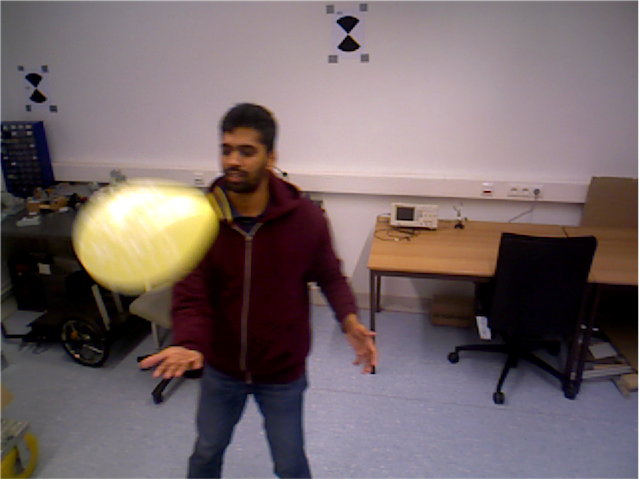
\includegraphics[width=\bonnfigwidth]{figure/analyses/comp_bonn/image.png} & 
 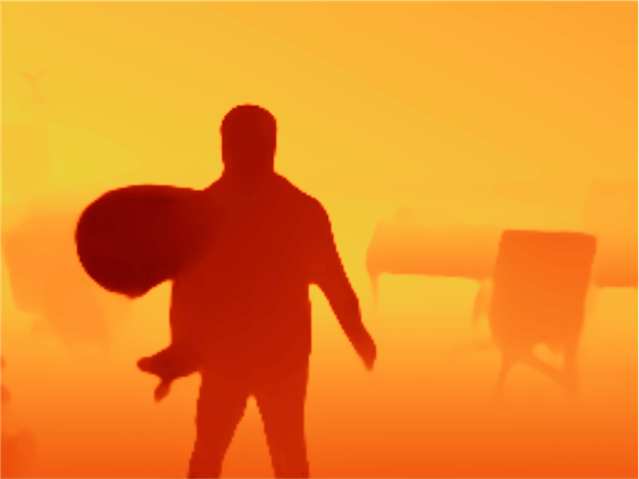
\includegraphics[width=\bonnfigwidth]{figure/analyses/comp_bonn/bonn_depth_dynadust3r.png} &
 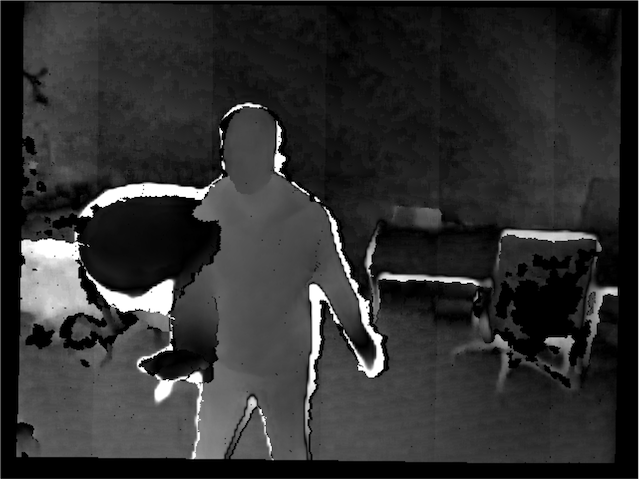
\includegraphics[width=\bonnfigwidth]{figure/analyses/comp_bonn/bonn_error_dynadust3r.png} &
 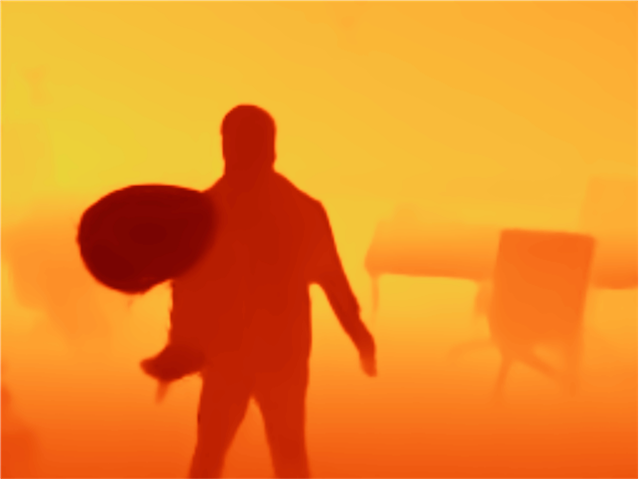
\includegraphics[width=\bonnfigwidth]{figure/analyses/comp_bonn/bonn_depth_ours.png} &
 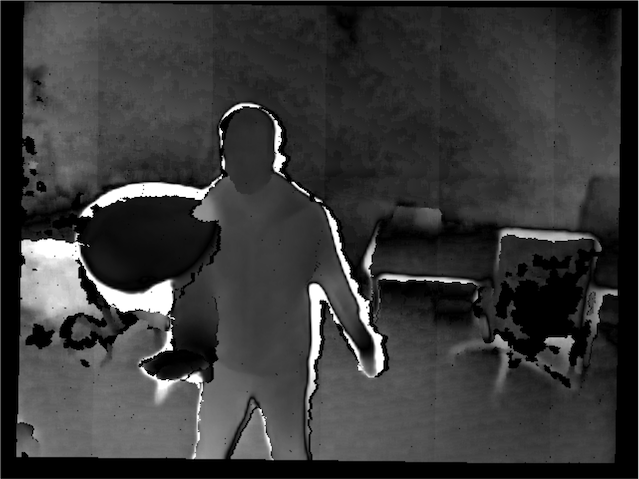
\includegraphics[width=\bonnfigwidth]{figure/analyses/comp_bonn/bonn_error_ours.png} \\
 Input image & Predicted depth & Error map & Predicted depth & Error map
\end{tabular}

\caption{
\textbf{Comparison with DynaDUSt3R on Bonn.} 
Unlike per-pixel point representation, our representation gives subtle inaccuracy in geometry on textureless region (\eg wall). Brighter means higher errors.
}
\label{fig:supp:bonn_error}
\end{figure*}


\subsection{Discussion on Bonn}
\label{supp:discussion_bonn}
While our method outperforms baselines across most benchmarks, its performance on the Bonn dataset is comparable to prior work (\cref{tab:exp:depth,tab:exp:architecture_comparison}).
We attribute this to the prevalence of textureless regions (\eg walls) in Bonn, where our model predicts large, highly overlapping Gaussians (\cref{fig:gaussian_scale}).
Although this overlap promotes surface continuity, it renders the point estimate dependent on a weighted combination of multiple Gaussians, making it susceptible to accumulated blending errors from nearby Gaussians.
In contrast, per-pixel representations (\eg DynaDUSt3R, MonST3R) avoid this spatial dependency by estimating depth in isolation.

Consequently, as visualized in \cref{fig:supp:bonn_error}, our method exhibits slightly higher errors in these textureless regions. We quantitatively confirm this hypothesis in \cref{tab:supp:scale_accuracy}, which demonstrates that depth accuracy degrades as the scale of the estimated 3D Gaussians increases.


\begin{table}[ht]
\centering
\scriptsize
\setlength\tabcolsep{2pt}
\caption{
\textbf{Impact of Gaussian scale on geometry accuracy on Bonn.} We report Point EPE and Depth Abs.~Rel. across different ranges of estimated Gaussian scales. We observe that depth accuracy decreases along with the increased scale of estimated 3D Gaussians.}
\label{tab:supp:scale_accuracy}
\newcolumntype{Y}{>{\centering\arraybackslash}X}
\begin{tabularx}{0.45\linewidth}{l @{\hskip 1em} YY}
\toprule
Scale Range & Point (EPE) $\downarrow$ & Depth (Abs. Rel.) $\downarrow$ \\
\midrule
$0 - 0.5$   & 0.189 & 0.073 \\
$0.5 - 1.0$ & 0.151 & 0.059 \\
$1.0 - 1.5$ & 0.200 & 0.068 \\
$1.5 - 2.0$ & 0.189 & 0.067 \\
$2.0 - 2.5$ & 0.185 & 0.071 \\
$2.5 - 3.0$ & 0.205 & 0.085 \\
\bottomrule
\end{tabularx}
\end{table}












\begin{figure*}[!t]
\centering
\scriptsize
\setlength\tabcolsep{0.2pt}

\newcommand{\qualimgjpg}[3]{\includegraphics[width=0.186\textwidth]{figure/analyses/cross_attention_camera/#1/#2/#3.jpg}}

\newcommand{\qualattenjpg}[4]{\includegraphics[width=0.186\textwidth]{figure/analyses/cross_attention_camera/#1/#2/#3_0.75_-0.75_#4.jpg}}


\newcommand{\carowdynamic}[2]{
\rotatebox{90}{Dynamic} & 
\qualimgjpg{dynamic}{#1}{img0} &
\qualimgjpg{dynamic}{#1}{img1} &
\qualattenjpg{dynamic}{#1}{#2}{07} &
\qualattenjpg{dynamic}{#1}{#2}{10} &
\qualattenjpg{dynamic}{#1}{#2}{11}
}

\newcommand{\carowstatic}[2]{
\rotatebox{90}{Static} & 
\qualimgjpg{static}{#1}{img0} &
\qualimgjpg{static}{#1}{img0} &
\qualattenjpg{static}{#1}{#2}{07} &
\qualattenjpg{static}{#1}{#2}{10} &
\qualattenjpg{static}{#1}{#2}{11}
}


\newcolumntype{M}{>{\centering\arraybackslash}m{0.186\textwidth}}
\newcolumntype{N}{>{\centering\arraybackslash}m{0.02\textwidth}}

\begin{tabular}{N @{\hspace{0.8em}} M M @{\hspace{0.8em}} M M M M}
    & \multicolumn{2}{c}{Input pair} & Block 8th & Block 11th & Block 12th \\
    \carowdynamic{rgbd_bonn_crowd2_1548339893.24032_1548339893.57482}{viz2} \\
    \carowstatic{rgbd_bonn_crowd2_1548339893.24032_1548339893.57482}{viz2} \\ \noalign{\smallskip}

    \carowdynamic{6nL_ifACgfE-clip0-frame_50_72}{viz2} \\
    \carowstatic{6nL_ifACgfE-clip0-frame_50_72}{viz2} \\ \noalign{\smallskip}

    \carowdynamic{market_5_0001_0002}{viz2} \\
    \carowstatic{market_5_0001_0002}{viz2} \\

\end{tabular}
    \caption{\textbf{Visualization of cross-attention maps of the camera pose token.} We observe that at specific blocks (Blocks 8th, 11th, and 12th), the camera pose token more attends to image tokens located in static regions (\ie, high attention scores in brighter colors), which provide reliable cues for relative camera pose estimation.
    Moving objects tend to have darker colors, \ie, lower attention scores.
    As a reference at each second row, we also visualize the cross-attention maps for a static scene configuration, where identical images are used as input.
    }
    \label{fig:supp:camera_token_atten}
\end{figure*}





\subsection{Cross-attention Map Visualization of the Camera Pose Token.}
\label{supp:cross_attn_viz}
Our method is capable of estimating accurate relative camera poses in scenes with dynamic objects.
To investigate the underlying mechanism enabling this robustness, we visualize the cross-attention maps between the learnable camera pose token and the image tokens in \cref{fig:supp:camera_token_atten}.
As a reference, we also visualize a static baseline for each scene by using two identical images as input.
We observe that at specific blocks (\eg the 8th, 11th, and 12th blocks), the cross-attention maps exhibit significantly higher attention scores in static regions, effectively suppressing attention on moving objects.



\begin{table}[t]
\centering
\scriptsize
\setlength\tabcolsep{3pt}
\caption{
\textbf{Ablation on Pose and Representation.} We compare our method with per-pixel baselines using different pose estimators (pose head vs. PnP-RANSAC). Our Dynamic 3DGS representation with the feedforward pose head achieves the best accuracy on Stereo4D and KITTI.
}
\label{tab:exp:pose_ablation}
\begin{tabularx}{0.85\linewidth}{@{}l X *{5}{S[table-format=1.3]} @{}}
\toprule
\multirow{2}{*}{Output representation} & \multirow{2}{*}{Pose estimator} & \multicolumn{2}{c}{Stereo4D} & \multicolumn{2}{c}{KITTI} & \multicolumn{1}{c}{Bonn} \\
\cmidrule(lr){3-4} \cmidrule(lr){5-6} \cmidrule(lr){7-7}
& & {Motion EPE} & {Point EPE} & {Motion EPE} & {Point EPE} & {Point EPE} \\
\midrule
Dynamic 3DGS (\textbf{Ours}) & Pose head & \bfseries 0.057 & \bfseries 0.781 & \bfseries 0.244 & \bfseries 3.553 & 0.211 \\ \midrule

\multirow{2}{*}{Per-pixel point and motion} & Pose head & 0.060 & 0.811 & 0.245 & 4.396 & 0.206 \\
 & PnP-RANSAC & 0.058 & 0.809 & 0.283 & 4.567 & \bfseries 0.196 \\
\bottomrule
\end{tabularx}
\end{table}






\begin{figure*}[t]
\centering
\scriptsize
\setlength\tabcolsep{0.2pt}
\newcommand{\qualimgpng}[3]{\includegraphics[width=0.23\textwidth]{figure/analyses/architecture_kitti/#1/#2_1_#3_view0.png}}

\newcommand{\archqualrowkitti}[1]{
\qualimgpng{img}{#1}{input} & 
\qualimgpng{img}{#1}{depth_target} & 
\rotatebox{90}{Pred.} &
\qualimgpng{ours}{#1}{depth_pred_rendered} & 
\qualimgpng{dynadust3r}{#1}{depth_pred_rendered} \\
 & 
 & 
\rotatebox{90}{Error} &
\qualimgpng{ours}{#1}{depth_error} & 
\qualimgpng{dynadust3r}{#1}{depth_error} 
}

\newcolumntype{M}{>{\centering\arraybackslash}m{0.23\textwidth}}
\newcolumntype{N}{>{\centering\arraybackslash}m{0.02\textwidth}}

\begin{tabular}{M M @{\hspace{0.8em}} N M M}
Image & Ground Truth & & \textbf{Ours} & Per-pixel representation \\ 
\archqualrowkitti{2} \\ \noalign{\smallskip}
\archqualrowkitti{22} \\ \noalign{\smallskip}
\archqualrowkitti{92} \\ \noalign{\smallskip}
\archqualrowkitti{103} \\ \noalign{\smallskip}
\archqualrowkitti{110} \\

\end{tabular}

\caption{
\textbf{Qualitative comparison of our method and baseline with per-pixel point representation on KITTI.} Unlike per-pixel representation model, our method yields much better accuracy especially on planar road surface, benefiting from our accurate pose estimation and photometric losses on rendered images. In error maps, darker means more accurate.
\label{fig:supp:qual_kitti_comp}
}
\end{figure*}


\subsection{Discussion on the Accuracy Gain on KITTI}
In \cref{tab:exp:architecture_comparison} in the main paper, our representation shows much better accuracy gain on KITTI, comparing to the model with per-pixel point and motion representation.
We find that the huge accuracy gain on KITTI is from both the accurate pose estimation and better supervision with our photometric losses.

Our accuracy gain for motion on KITTI primarily originates from our accurate pose estimation.
Since KITTI evaluates motion in local camera coordinates, predictions in the canonical camera coordinate need to be transformed using estimated poses.
For baselines, we use PnP-RANSAC that follows their formulation.
In contrast, Our method utilizes a significantly more accurate, directly estimated feedforward pose, leading better motion accuracy in the end.
We validated this source of improvement by training a per-pixel baseline equipped with a pose head (\ie equivalent to DynaDUSt3R with the pose head.).
As in \cref{tab:exp:pose_ablation}, its motion accuracy on KITTI now almost matches our method, highlighting the importance of the our feedforward pose estimation.

For gain on point accuracy, we attribute the gain to the photometric loss acting as an additional dense supervision signal, which also gets benefits from our robust pose estimation.
\cref{fig:supp:qual_kitti_comp} shows that our representation has much lower errors on planar road areas comparing to the model with per-pixel representation.
With an accurate pose, the loss on the rasterized image effectively encourages the model to respect multi-view stereo constraints, guiding the estimated point to be geometrically consistent with the parallax in both views.
This allows the model to better leverage both images as geometric supervision, whereas baselines only have view-independent sparse per-point supervision.


\subsection{Discussion on the Better Pose Accuracy}
\label{sec:supp:pose_pnp}

\cref{tab:exp:pose} in the main paper demonstrates that our method achieves the best pose accuracy among direct competitors.
We further investigate the source of the gain to determine whether it originates from our feedforward estimation or the improved geometry. 
To answer the question, we also estimate relative pose via PnP+RANSAC from our predicted Gaussian centers.

The answer is both. As in \cref{tab:exp:pose_pnp}, our method with PnP with RANSAC still substantially outperforms other methods.
This validates the higher accuracy of our estimated geometry than others, indicating that estimated points are aligned well with direction of each camera ray.
Furthermore, our direct feedforward estimator achieves $\sim$16.6\% higher accuracy than this PnP baseline, further demonstrating its robustness over noise-sensitive iterative solvers.

\begin{table}[t]
\centering
\scriptsize
\setlength\tabcolsep{3pt}
\caption{\textbf{Pose estimation with PnP+RANSAC.}
Our method with PnP+RANSAC also outperforms direct competitors, validating the higher accuracy of our estimated geometry than others.
Also our direct feedforward estimator achieves $\sim$16.6\% higher accuracy than this baseline, further demonstrating its robustness over noise-sensitive iterative solvers.
ATE and RPE translation ($\text{RPE}_\text{trans}$) and rotation ($\text{RPE}_\text{rot}$) are reported.
}
\label{tab:exp:pose_pnp}
\newcolumntype{Y}{S[table-format=2.4, round-mode=places, round-precision=4]}
\newcolumntype{Z}{S[table-format=2.3, round-mode=places, round-precision=3]}
\begin{tabularx}{\linewidth}{@{} X @{\hskip 2em} *{3}{Y Y Z} @{}}
\toprule
\multirow{2}{*}{Method} & \multicolumn{3}{c}{Stereo4D \citep{Jin:2025:S4D}} & \multicolumn{3}{c}{Bonn~\citep{Palazzolo:2019:RF3}} &
\multicolumn{3}{c}{Sintel~\citep{Butler:2012:ANO}} \\ \cmidrule(lr){2-4} \cmidrule(lr){5-7} \cmidrule(lr){8-10}
& {$\text{ATE}$} & {$\text{RPE}_\text{trans}$} & {$\text{RPE}_\text{rot}$} & {$\text{ATE}$} & {$\text{RPE}_\text{trans}$} & {$\text{RPE}_\text{rot}$} & {$\text{ATE}$} & {$\text{RPE}_\text{trans}$} & {$\text{RPE}_\text{rot}$} \\
\midrule
MonST3R~\citep{Zhang:2025:MST} & 0.0458 & 0.0647 & 0.8047 & 0.0031 & 0.0043 & 0.5436 & 0.0290 & 0.0410 & 1.0796 \\
St4RTrack~\citep{Feng:2025:ST4} & 0.0602 & 0.0851 & 0.7289 & 0.0024 & 0.0034 & 0.3997 & 0.0231 & 0.0326 & 0.8835 \\
\ourmethod{} (Ours, with PnP+RANSAC) & 0.0120 & 0.0170 & 0.2052 & 0.0024 & 0.0033 & 0.2933 & 0.0168 & 0.0238 & 0.3315 \\
\midrule
\textbf{\ourmethod{} (Ours, with the pose head)} & \bfseries 0.0101 & \bfseries 0.0142 & \bfseries 0.1794 & \bfseries 0.0020 & \bfseries 0.0028 & \bfseries 0.2709 & \bfseries 0.0122 & \bfseries 0.0172 & \bfseries 0.2980 \\
\bottomrule
\end{tabularx}
\end{table}

                                    

\paragraph{The usage of Large Language Models (LLMs) in paper writing.} The paper got helps from LLMs for polishing writing and grammar correction.

